\section{内部飛跡検出器}

\begin{figure}[h]   %*** 図を分割して表示することができる
    \begin{minipage}[b]{0.5\linewidth}
        \centering
        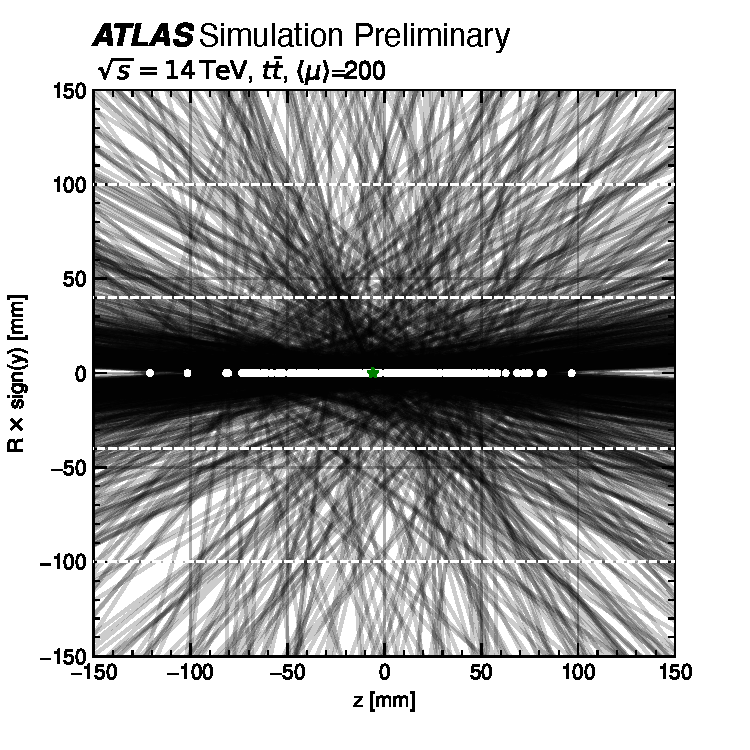
\includegraphics[scale=0.5]{fig/ch1/ATLAS_3Dtrack.pdf}
        \subcaption{位置分解能による飛跡の再構成}
        \label{fg:ATLAS_3Dtrack}
    \end{minipage}
    \begin{minipage}[b]{0.5\linewidth}
        \centering
        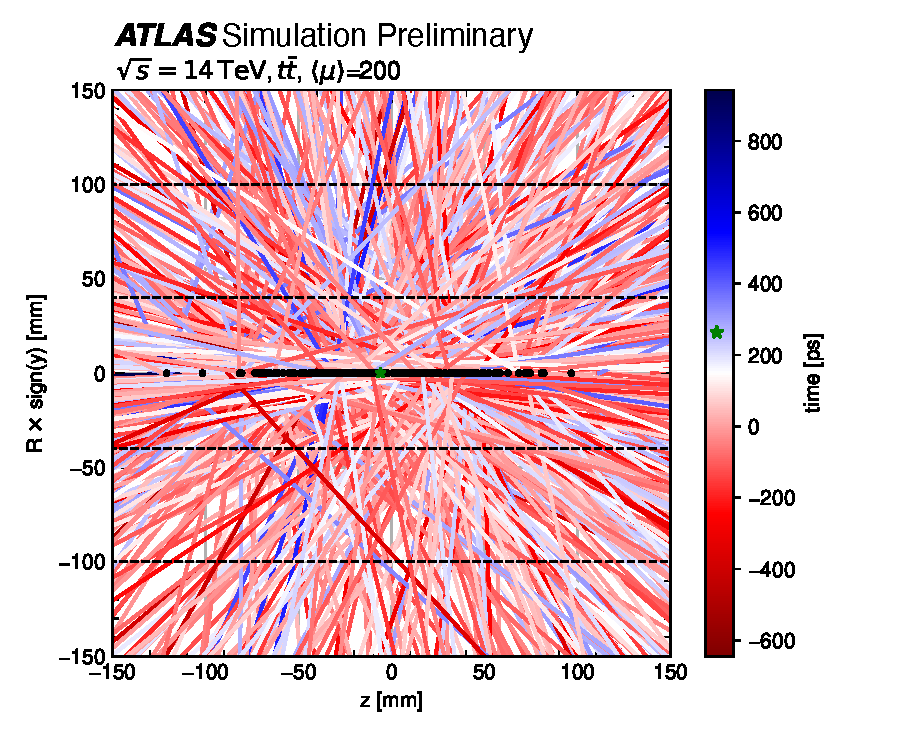
\includegraphics[scale=0.5]{fig/ch1/ATLAS_4Dtrack.pdf}
        \subcaption{位置分解能と時間分解能による飛跡の再構成}
        \label{fg:ATLAS_4Dtrack}
    \end{minipage}
    \caption[飛跡の再構成のシミュレーション\cite{ATL-PHYS-PUB-2023-023}]{飛跡の再構成のシミュレーション\cite{ATL-PHYS-PUB-2023-023}\\時間分解能があることで、衝突点と飛跡がどのタイミングで起こったのかがわかる。粒子密度が高くなっても衝突点と飛跡の紐付けが可能。}
    \label{fg:4Dtrack_ATLAS}
\end{figure}


